\newread\ktlsevalfile%

\newcommand{\IfNonemptyKtlsEvalFile}[3]{%
    \IfFileExists{#1}{%
        \openin\ktlsevalfile=#1
        \ifeof\ktlsevalfile%
            \closein\ktlsevalfile%
            #3%
        \else
            \closein\ktlsevalfile%
            #2%
        \fi
    }{%
        #3%
    }%
}

\newcommand{\KtlsEvalPlot}[3]{%
    \IfNonemptyKtlsEvalFile{#3}{%
        \addplot+[#1]
        table [#2, col sep=comma] {#3};
    }{}%
}

\newcommand{\KtlsEvalHundredUsSchedsimPlot}[1]{%
    \KtlsEvalPlot{mark=none, solid, cLightBlue}{x expr=\thisrow{Req/time_unit} * 10000, y expr=\thisrow{99th (us)} / 10}{data/schedsim/single_queue/FIFO_1000_20_80_#1.csv}%
}

\newcommand{\KtlsEvalTwentyUsSchedsimPlot}[1]{%
    \KtlsEvalPlot{mark=none, solid, cLightBlue}{x expr=\thisrow{Req/time_unit} * 50000, y expr=\thisrow{99th (us)} / 50}{data/schedsim/single_queue/FIFO_1000_20_80_#1.csv}%
}

\newcommand{\KtlsEvalYAxisStyle}{%
    scaled y ticks=false,
    ytick={200, 400, 600, 800, 1000},
    yticklabel style={
        /pgf/number format/fixed,
        /pgf/number format/precision=0,
    }%
}

\newcommand{\KtlsEvalPanelWidth}{5.69cm}

\begin{figure*}[!t]
    \centering
    \captionsetup[subfigure]{justification=centering,singlelinecheck=false,width=\KtlsEvalPanelWidth}
    \begin{minipage}{\linewidth}
        \centering
        \begin{subfigure}[b]{\KtlsEvalPanelWidth}
            \centering
            \begin{tikzpicture} [scale=0.875, transform shape, trim axis left, trim axis right]
                \begin{axis}
                    [
                        xlabel={Load (KQPS)},
                        ylabel={Latency (\si{\micro\second})},
                        xmin=0,
                        xmax=200,
                        ymin=0,
                        ymax=1000,
                        enlarge y limits=false,
                        restrict x to domain*=0:5E9,
                        restrict y to domain*=0:1E4,
                        \KtlsEvalYAxisStyle,
                        axis y line=left,
                        axis x line=bottom,
                        height=3.9cm,
                        width=6.5cm,
                        legend cell align=left,
                        legend style={
                            draw=none,
                            font=\footnotesize,
                            anchor=south,
                            at={(0.78, 1.15)},
                            legend columns=2,
                            /tikz/every even column/.append style={column sep=0.45cm},
                        },
                    ]
                    \addlegendimage{floating_tlsStyle}
                    \addlegendentry{TCP-CS-80 TLS}

                    \addlegendimage{floatingStyle}
                    \addlegendentry{TCP-CS-80}

                    \KtlsEvalPlot{
                        workerPoolStyle,
                        x filter/.code={
                            \IfStrEq{\thisrow{dist_config}}{fixed}{}{\def\pgfmathresult{}}
                        }
                    }{x expr=\thisrow{load_pool(QPS)} / 1000, y=latency_pool}{data/synthetic_80_100us.csv}

                    \KtlsEvalPlot{
                        workerPool_tlsStyle,
                        x filter/.code={
                            \IfStrEq{\thisrow{dist_config}}{fixed}{}{\def\pgfmathresult{}}
                        }
                    }{x expr=\thisrow{load_pool-tls(QPS)} / 1000, y=latency_pool-tls}{data/ktls_100us.csv}

                    \KtlsEvalPlot{
                        floatingStyle,
                        x filter/.code={
                            \IfStrEq{\thisrow{dist_config}}{fixed}{}{\def\pgfmathresult{}}
                        }
                    }{x expr=\thisrow{load_floating(QPS)} / 1000, y=latency_floating}{data/synthetic_80_100us.csv}

                    \KtlsEvalPlot{
                        floating_tlsStyle,
                        x filter/.code={
                            \IfStrEq{\thisrow{dist_config}}{fixed}{}{\def\pgfmathresult{}}
                        }
                    }{x expr=\thisrow{load_floating-tls(QPS)} / 1000, y=latency_floating-tls}{data/ktls_100us.csv}

                    \KtlsEvalPlot{
                        koma_tlsStyle,
                        x filter/.code={
                            \IfStrEq{\thisrow{dist_config}}{fixed}{}{\def\pgfmathresult{}}
                        }
                    }{x expr=\thisrow{load_koma-tls(QPS)} / 1000, y=latency_koma-tls}{data/ktls_100us.csv}

                    \KtlsEvalPlot{
                        komaStyle,
                        x filter/.code={
                            \IfStrEq{\thisrow{dist_config}}{fixed}{}{\def\pgfmathresult{}}
                        }
                    }{x expr=\thisrow{load_koma(QPS)} / 1000, y=latency_koma}{data/synthetic_80_100us.csv}

                    \KtlsEvalHundredUsSchedsimPlot{d}
                \end{axis}
            \end{tikzpicture}
            \caption{\add{Fixed ($\bar{S}=100\si{\micro\second}$).}}
        \end{subfigure}
        \hfill
        \begin{subfigure}[b]{\KtlsEvalPanelWidth}
            \centering
            \begin{tikzpicture} [scale=0.875, transform shape, trim axis left, trim axis right]
                \begin{axis}
                    [
                        xlabel={Load (KQPS)},
                        ylabel style={opacity=0},
                        ylabel={\phantom{Latency}},
                        xmin=0,
                        xmax=200,
                        ymin=0,
                        ymax=1000,
                        enlarge y limits=false,
                        restrict x to domain*=0:5E9,
                        restrict y to domain*=0:1E4,
                        \KtlsEvalYAxisStyle,
                        axis y line=left,
                        axis x line=bottom,
                        height=3.9cm,
                        width=6.5cm,
                        legend cell align=left,
                        legend style={
                            draw=none,
                            font=\footnotesize,
                            anchor=south,
                            at={(0.48, 1.15)},
                            legend columns=2,
                            /tikz/every even column/.append style={column sep=0.45cm},
                        },
                    ]

                    \addlegendimage{workerPool_tlsStyle}
                    \addlegendentry{Worker Pool TLS}

                    \addlegendimage{workerPoolStyle}
                    \addlegendentry{Worker Pool}

                    \KtlsEvalPlot{
                        workerPoolStyle,
                        x filter/.code={
                            \IfStrEq{\thisrow{dist_config}}{exponential}{}{\def\pgfmathresult{}}
                        }
                    }{x expr=\thisrow{load_pool(QPS)} / 1000, y=latency_pool}{data/synthetic_80_100us.csv}

                    \KtlsEvalPlot{
                        workerPool_tlsStyle,
                        x filter/.code={
                            \IfStrEq{\thisrow{dist_config}}{exponential}{}{\def\pgfmathresult{}}
                        }
                    }{x expr=\thisrow{load_pool-tls(QPS)} / 1000, y=latency_pool-tls}{data/ktls_100us.csv}

                    \KtlsEvalPlot{
                        floatingStyle,
                        x filter/.code={
                            \IfStrEq{\thisrow{dist_config}}{exponential}{}{\def\pgfmathresult{}}
                        }
                    }{x expr=\thisrow{load_floating(QPS)} / 1000, y=latency_floating}{data/synthetic_80_100us.csv}

                    \KtlsEvalPlot{
                        floating_tlsStyle,
                        x filter/.code={
                            \IfStrEq{\thisrow{dist_config}}{exponential}{}{\def\pgfmathresult{}}
                        }
                    }{x expr=\thisrow{load_floating-tls(QPS)} / 1000, y=latency_floating-tls}{data/ktls_100us.csv}

                    \KtlsEvalPlot{
                        koma_tlsStyle,
                        x filter/.code={
                            \IfStrEq{\thisrow{dist_config}}{exponential}{}{\def\pgfmathresult{}}
                        }
                    }{x expr=\thisrow{load_koma-tls(QPS)} / 1000, y=latency_koma-tls}{data/ktls_100us.csv}

                    \KtlsEvalPlot{
                        komaStyle,
                        x filter/.code={
                            \IfStrEq{\thisrow{dist_config}}{exponential}{}{\def\pgfmathresult{}}
                        }
                    }{x expr=\thisrow{load_koma(QPS)} / 1000, y=latency_koma}{data/synthetic_80_100us.csv}

                    \KtlsEvalHundredUsSchedsimPlot{m}
                \end{axis}
            \end{tikzpicture}
            \caption{\add{Exponential ($\bar{S}=100\si{\micro\second}$).}}
        \end{subfigure}
        \hfill
        \begin{subfigure}[b]{\KtlsEvalPanelWidth}
            \centering
            \begin{tikzpicture} [scale=0.875, transform shape, trim axis left, trim axis right]
                \begin{axis}
                    [
                        xlabel={Load (KQPS)},
                        ylabel style={opacity=0},
                        ylabel={\phantom{Latency}},
                        xmin=0,
                        xmax=200,
                        ymin=0,
                        ymax=1000,
                        enlarge y limits=false,
                        restrict x to domain*=0:5E9,
                        restrict y to domain*=0:1E4,
                        \KtlsEvalYAxisStyle,
                        axis y line=left,
                        axis x line=bottom,
                        height=3.9cm,
                        width=6.5cm,
                        legend cell align=left,
                        legend style={
                            draw=none,
                            font=\footnotesize,
                            anchor=south,
                            at={(0.35, 1.15)},
                            legend columns=3,
                            /tikz/every even column/.append style={column sep=0.45cm},
                        },
                    ]
                    \addlegendimage{koma_tlsStyle}
                    \addlegendentry{\system-kTLS}

                    \addlegendimage{komaStyle}
                    \addlegendentry{\system}

                    \addlegendimage{mark=none, solid, cLightBlue}
                    \addlegendentry{MS}

                    \KtlsEvalPlot{
                        workerPoolStyle,
                        x filter/.code={
                            \IfStrEq{\thisrow{dist_config}}{bimodal}{}{\def\pgfmathresult{}}
                        }
                    }{x expr=\thisrow{load_pool(QPS)} / 1000, y=latency_pool}{data/synthetic_80_100us.csv}

                    \KtlsEvalPlot{
                        workerPool_tlsStyle,
                        x filter/.code={
                            \IfStrEq{\thisrow{dist_config}}{bimodal}{}{\def\pgfmathresult{}}
                        }
                    }{x expr=\thisrow{load_pool-tls(QPS)} / 1000, y=latency_pool-tls}{data/ktls_100us.csv}

                    \KtlsEvalPlot{
                        floatingStyle,
                        x filter/.code={
                            \IfStrEq{\thisrow{dist_config}}{bimodal}{}{\def\pgfmathresult{}}
                        }
                    }{x expr=\thisrow{load_floating(QPS)} / 1000, y=latency_floating}{data/synthetic_80_100us.csv}

                    \KtlsEvalPlot{
                        floating_tlsStyle,
                        x filter/.code={
                            \IfStrEq{\thisrow{dist_config}}{bimodal}{}{\def\pgfmathresult{}}
                        }
                    }{x expr=\thisrow{load_floating-tls(QPS)} / 1000, y=latency_floating-tls}{data/ktls_100us.csv}

                    \KtlsEvalPlot{
                        koma_tlsStyle,
                        x filter/.code={
                            \IfStrEq{\thisrow{dist_config}}{bimodal}{}{\def\pgfmathresult{}}
                        }
                    }{x expr=\thisrow{load_koma-tls(QPS)} / 1000, y=latency_koma-tls}{data/ktls_100us.csv}

                    \KtlsEvalPlot{
                        komaStyle,
                        x filter/.code={
                            \IfStrEq{\thisrow{dist_config}}{bimodal}{}{\def\pgfmathresult{}}
                        }
                    }{x expr=\thisrow{load_koma(QPS)} / 1000, y=latency_koma}{data/synthetic_80_100us.csv}

                    \KtlsEvalHundredUsSchedsimPlot{b}
                \end{axis}
            \end{tikzpicture}
            \caption{\add{Bimodal ($\bar{S}=100\si{\micro\second}$).}}
        \end{subfigure}
    \end{minipage}

    \begin{minipage}{\linewidth}
        \centering
        \begin{subfigure}[b]{\KtlsEvalPanelWidth}
            \centering
            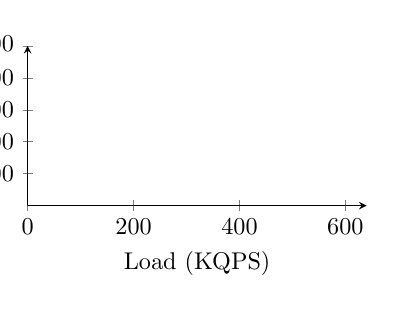
\begin{tikzpicture} [scale=0.875, transform shape, trim axis left, trim axis right]
                \begin{axis}
                    [
                        xlabel={Load (KQPS)},
                        ylabel={Latency (\si{\micro\second})},
                        xmin=0,
                        xmax=640,
                        ymin=0,
                        ymax=1000,
                        enlarge y limits=false,
                        restrict x to domain*=0:5E9,
                        restrict y to domain*=0:1E4,
                        \KtlsEvalYAxisStyle,
                        axis y line=left,
                        axis x line=bottom,
                        height=3.9cm,
                        width=6.5cm,
                        legend cell align=left,
                    ]
                    \KtlsEvalPlot{
                        workerPoolStyle,
                        x filter/.code={
                            \IfStrEq{\thisrow{dist_config}}{fixed}{}{\def\pgfmathresult{}}
                        }
                    }{x expr=\thisrow{load_pool(QPS)} / 1000, y=latency_pool}{data/synthetic_80_20us.csv}

                    \KtlsEvalPlot{
                        workerPool_tlsStyle,
                        x filter/.code={
                            \IfStrEq{\thisrow{dist_config}}{fixed}{}{\def\pgfmathresult{}}
                        }
                    }{x expr=\thisrow{load_pool-tls(QPS)} / 1000, y=latency_pool-tls}{data/ktls_20us.csv}

                    \KtlsEvalPlot{
                        floatingStyle,
                        x filter/.code={
                            \IfStrEq{\thisrow{dist_config}}{fixed}{}{\def\pgfmathresult{}}
                        }
                    }{x expr=\thisrow{load_floating(QPS)} / 1000, y=latency_floating}{data/synthetic_80_20us.csv}

                    \KtlsEvalPlot{
                        floating_tlsStyle,
                        x filter/.code={
                            \IfStrEq{\thisrow{dist_config}}{fixed}{}{\def\pgfmathresult{}}
                        }
                    }{x expr=\thisrow{load_floating-tls(QPS)} / 1000, y=latency_floating-tls}{data/ktls_20us.csv}

                    \KtlsEvalPlot{
                        koma_tlsStyle,
                        x filter/.code={
                            \IfStrEq{\thisrow{dist_config}}{fixed}{}{\def\pgfmathresult{}}
                        }
                    }{x expr=\thisrow{load_koma-tls(QPS)} / 1000, y=latency_koma-tls}{data/ktls_20us.csv}

                    \KtlsEvalPlot{
                        komaStyle,
                        x filter/.code={
                            \IfStrEq{\thisrow{dist_config}}{fixed}{}{\def\pgfmathresult{}}
                        }
                    }{x expr=\thisrow{load_koma(QPS)} / 1000, y=latency_koma}{data/synthetic_80_20us.csv}

                    \KtlsEvalTwentyUsSchedsimPlot{d}
                \end{axis}
            \end{tikzpicture}
            \caption{\add{Fixed ($\bar{S}=20\si{\micro\second}$).}}
        \end{subfigure}
        \hfill
        \begin{subfigure}[b]{\KtlsEvalPanelWidth}
            \centering
            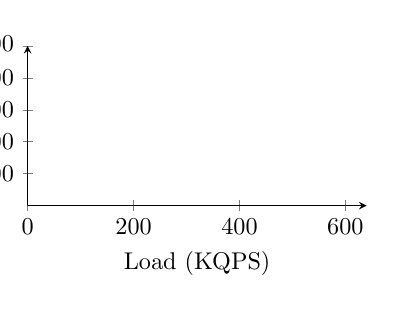
\begin{tikzpicture} [scale=0.875, transform shape, trim axis left, trim axis right]
                \begin{axis}
                    [
                        xlabel={Load (KQPS)},
                        ylabel style={opacity=0},
                        ylabel={\phantom{Latency}},
                        xmin=0,
                        xmax=640,
                        ymin=0,
                        ymax=1000,
                        enlarge y limits=false,
                        restrict x to domain*=0:5E9,
                        restrict y to domain*=0:1E4,
                        \KtlsEvalYAxisStyle,
                        axis y line=left,
                        axis x line=bottom,
                        height=3.9cm,
                        width=6.5cm,
                        legend cell align=left,
                    ]
                    \KtlsEvalPlot{
                        workerPoolStyle,
                        x filter/.code={
                            \IfStrEq{\thisrow{dist_config}}{exponential}{}{\def\pgfmathresult{}}
                        }
                    }{x expr=\thisrow{load_pool(QPS)} / 1000, y=latency_pool}{data/synthetic_80_20us.csv}

                    \KtlsEvalPlot{
                        workerPool_tlsStyle,
                        x filter/.code={
                            \IfStrEq{\thisrow{dist_config}}{exponential}{}{\def\pgfmathresult{}}
                        }
                    }{x expr=\thisrow{load_pool-tls(QPS)} / 1000, y=latency_pool-tls}{data/ktls_20us.csv}

                    \KtlsEvalPlot{
                        floatingStyle,
                        x filter/.code={
                            \IfStrEq{\thisrow{dist_config}}{exponential}{}{\def\pgfmathresult{}}
                        }
                    }{x expr=\thisrow{load_floating(QPS)} / 1000, y=latency_floating}{data/synthetic_80_20us.csv}

                    \KtlsEvalPlot{
                        floating_tlsStyle,
                        x filter/.code={
                            \IfStrEq{\thisrow{dist_config}}{exponential}{}{\def\pgfmathresult{}}
                        }
                    }{x expr=\thisrow{load_floating-tls(QPS)} / 1000, y=latency_floating-tls}{data/ktls_20us.csv}

                    \KtlsEvalPlot{
                        koma_tlsStyle,
                        x filter/.code={
                            \IfStrEq{\thisrow{dist_config}}{exponential}{}{\def\pgfmathresult{}}
                        }
                    }{x expr=\thisrow{load_koma-tls(QPS)} / 1000, y=latency_koma-tls}{data/ktls_20us.csv}

                    \KtlsEvalPlot{
                        komaStyle,
                        x filter/.code={
                            \IfStrEq{\thisrow{dist_config}}{exponential}{}{\def\pgfmathresult{}}
                        }
                    }{x expr=\thisrow{load_koma(QPS)} / 1000, y=latency_koma}{data/synthetic_80_20us.csv}

                    \KtlsEvalTwentyUsSchedsimPlot{m}
                \end{axis}
            \end{tikzpicture}
            \caption{\add{Exponential ($\bar{S}=20\si{\micro\second}$).}}
        \end{subfigure}
        \hfill
        \begin{subfigure}[b]{\KtlsEvalPanelWidth}
            \centering
            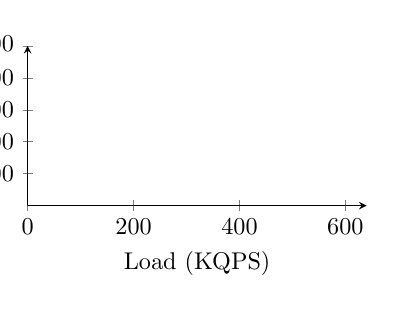
\begin{tikzpicture} [scale=0.875, transform shape, trim axis left, trim axis right]
                \begin{axis}
                    [
                        xlabel={Load (KQPS)},
                        ylabel style={opacity=0},
                        ylabel={\phantom{Latency}},
                        xmin=0,
                        xmax=640,
                        ymin=0,
                        ymax=1000,
                        enlarge y limits=false,
                        restrict x to domain*=0:5E9,
                        restrict y to domain*=0:1E4,
                        \KtlsEvalYAxisStyle,
                        axis y line=left,
                        axis x line=bottom,
                        height=3.9cm,
                        width=6.5cm,
                        legend cell align=left,
                    ]
                    \KtlsEvalPlot{
                        workerPoolStyle,
                        x filter/.code={
                            \IfStrEq{\thisrow{dist_config}}{bimodal}{}{\def\pgfmathresult{}}
                        }
                    }{x expr=\thisrow{load_pool(QPS)} / 1000, y=latency_pool}{data/synthetic_80_20us.csv}

                    \KtlsEvalPlot{
                        workerPool_tlsStyle,
                        x filter/.code={
                            \IfStrEq{\thisrow{dist_config}}{bimodal}{}{\def\pgfmathresult{}}
                        }
                    }{x expr=\thisrow{load_pool-tls(QPS)} / 1000, y=latency_pool-tls}{data/ktls_20us.csv}

                    \KtlsEvalPlot{
                        floatingStyle,
                        x filter/.code={
                            \IfStrEq{\thisrow{dist_config}}{bimodal}{}{\def\pgfmathresult{}}
                        }
                    }{x expr=\thisrow{load_floating(QPS)} / 1000, y=latency_floating}{data/synthetic_80_20us.csv}

                    \KtlsEvalPlot{
                        floating_tlsStyle,
                        x filter/.code={
                            \IfStrEq{\thisrow{dist_config}}{bimodal}{}{\def\pgfmathresult{}}
                        }
                    }{x expr=\thisrow{load_floating-tls(QPS)} / 1000, y=latency_floating-tls}{data/ktls_20us.csv}

                    \KtlsEvalPlot{
                        koma_tlsStyle,
                        x filter/.code={
                            \IfStrEq{\thisrow{dist_config}}{bimodal}{}{\def\pgfmathresult{}}
                        }
                    }{x expr=\thisrow{load_koma-tls(QPS)} / 1000, y=latency_koma-tls}{data/ktls_20us.csv}

                    \KtlsEvalPlot{
                        komaStyle,
                        x filter/.code={
                            \IfStrEq{\thisrow{dist_config}}{bimodal}{}{\def\pgfmathresult{}}
                        }
                    }{x expr=\thisrow{load_koma(QPS)} / 1000, y=latency_koma}{data/synthetic_80_20us.csv}

                    \KtlsEvalTwentyUsSchedsimPlot{b}
                \end{axis}
            \end{tikzpicture}
            \caption{\add{Bimodal ($\bar{S}=20\si{\micro\second}$).}}
        \end{subfigure}
    \end{minipage}
    \caption{\add{\nineninepct{} latency as a function of throughput with TLS enabled.
    Top and bottom rows correspond to 100\si{\micro\second} and 20\si{\micro\second} tasks, respectively.}}\label{fig:ktls_eval}
    \vspace{-0.5em}
\end{figure*}
